\documentclass[12pt,a4paper]{article}
\usepackage[utf8]{inputenc}
\usepackage[english]{babel}
\usepackage{graphicx}
\author{Madhur Singhal\\2015CS10235}

\title{Parallel Prefix Sum}
\date{26 February, 2018}
\begin{document}
\maketitle
\section{Introduction}
The prefix sum, also called a scan, of a sequence of numbers $x_0$, $x_1$, $x_2$, $...$ is a second sequence of numbers $y_0$, $y_1$, $y_2$, $...$ denoting the sums of prefixes (running totals) of the input sequence at every index.
$$ y_0 = x_0$$
$$ y_1 = x_0 +x_1$$
$$y_2 = x_0 + x_1 +x_2$$
$$ ....$$
In addition to being a useful building block, the prefix sums operation is a good example of a co mputation that
seems inherently sequential, but for which there is an efficient parallel algorithm. In this assignment we implement a work efficient version of the prefix sum algorithm and analyze it's runtime.
\section{Implementation and Design Decisions}
The algorithm used by me is presented below.
\begin{enumerate}
\item Assign equal length contiguous chunks of the input array to each thread and have each thread compute the prefix sums over their own subarray.
\item Use $log(n)$ phases to compute a global prefix sum over the final values produced by each thread. This is done in a sort of tree like sweep way. After each phase use a barrier to allow threads to synchronize.
\item Use the global sum array as offsets for the local sums produced by each thread to get the final array. This means that thread 3's prefix sums are augmented by the global sum upto thread 2 to get the actual prefix sum.
\end{enumerate}
I used a total of three additional arrays, one to store the output and two additonal arrays to store the temporary results of the phases in between. OpenMP "for","barrier" ,"single" and "schedule" clauses were utilized. One design decision was to use a padding of 7 integers with every integer so that false sharing is avoided. Also barriers were used at some places to ensure correctness of code.
\section{Analysis}
As can be seen from the graphs the speedup is highest for 4 parallel elements(threads). Overall the efficiency is not good and well below the optimal.
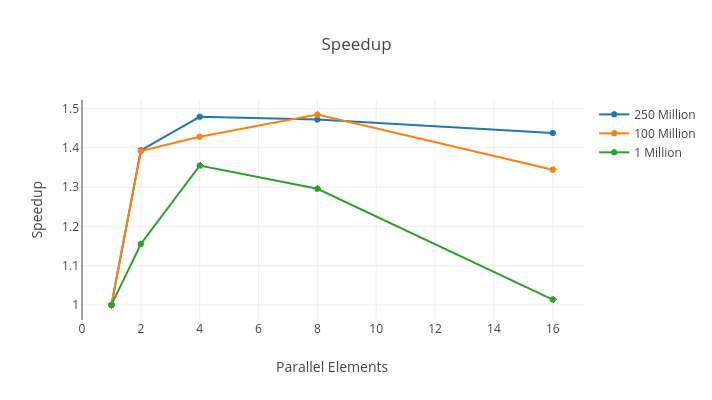
\includegraphics[scale=0.54]{spd}\\
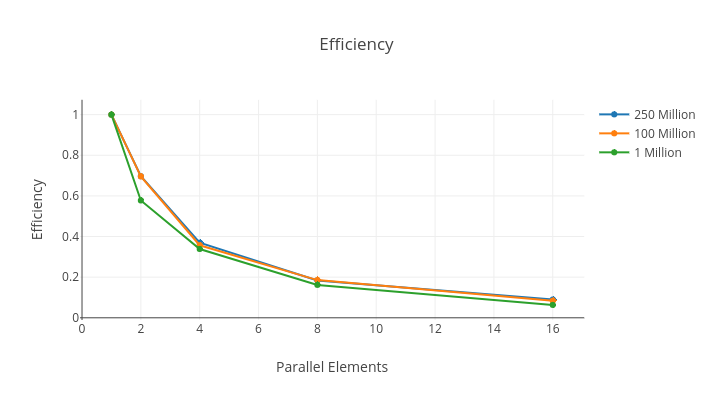
\includegraphics[scale=0.54]{eff}
\section{Conclusion}
Thus our parallel implementation clearly performs better than the serial one in terms of wall clock time. This implementation is not too good in terms of efficiency as can be gleaned from the graph. This is due to the complexity of the summation in phases (using barriers).
\end{document}